\documentclass[a4paper,10pt,headlines=3.2]{scrartcl}

%F�r Windows:
%\usepackage[T1]{fontenc}		%Umlaute
%\usepackage[latin1]{inputenc}		%latin-Zeichensatz

%\usepackage[colorlinks]{hyperref}	%Hyperlinks + Verlinkung innerhalb von PDFs

\usepackage{ucs}			%Formatierung (Linux)
\usepackage{graphicx}           	%Bilder
\usepackage[ngerman]{babel}		%Deutsche Sprache
\usepackage{amsmath}			%Math. Zeichen
\usepackage{pifont}			%Skalierbare Schriftart
\usepackage{array}			%Arrays
\usepackage{epsfig}			%Erweiterte Grafiken
\usepackage{makeidx}			%Stichwortverzeichnis
\usepackage[pdftex]{color} 		%Farbige PDFs
\newcommand{\changefont}[3]{    	%Definition von Schriftarten
\fontfamily{#1} \fontseries{#2} \fontshape{#3} \selectfont}
\makeindex				%Inhaltsverzeichnis erstellen
\usepackage[automark]{scrpage2}		%scrpage
\usepackage[nosectionbib]{apacite}	%Zitieren nach APA
\usepackage{lmodern}			%Font: Latin modern
\usepackage{scrpage2}           	%KOMA-Script
\usepackage{tipa}			%Phonologische Symbole
\usepackage{qtree}			%Baumstrukturen
\usepackage{pgf}			%Rastergrafiken
\usepackage{remreset}			%Fussnoten global
\makeatletter				
\@removefromreset{footnote}{chapter}	
\makeatother 				
\setcounter{tocdepth}{3}		%Inhaltsverzeichnis bis auf Tiefe 3 ausgeben
\pagestyle{scrheadings}         	%Kopfzeilen: Seitenstil scrheadings verwenden
\changefont{cmss}{m}{n}			%Schriftart: Computer-Schrift
\usepackage{listings}			%Java-Quellcode ausgeben
\lstset{numbers=left, numberstyle=\tiny, numbersep=5pt} \lstset{language=Java} 


%Manuelle Einstellung der Seitengr�sse. Sonst automatisch, siehe unten.
%\setlength{\textheight}{24cm}
%\setlength{\textwidth}{16cm}
%\setlength{\topmargin}{-2cm}
%\setlength{\oddsidemargin}{0cm}

% Groesse des Textbereiches in der Seite
\setlength{\textwidth}{16cm}
\setlength{\textheight}{22cm}
% Kopf- und Fusszeile, Hoehe und Abstand vom Text
\setlength{\headheight}{15pt}
\setlength{\headsep}{0.8cm}

%----------- wird automatisch berechnet
% Linker Seiteneinzug
\setlength{\oddsidemargin}{2.5cm} \addtolength{\oddsidemargin}{-1in}
\setlength{\evensidemargin}{2.5cm} \addtolength{\evensidemargin}{-1in}
% Andere Groessen ausrechnen (vertikal zentrieren)
\setlength{\footskip}{\headsep}
\addtolength{\footskip}{\headheight}
\setlength{\topmargin}{\paperheight}
\addtolength{\topmargin}{-\textheight}
\addtolength{\topmargin}{-\headheight}
\addtolength{\topmargin}{-\headsep}
\addtolength{\topmargin}{-\footskip}
\addtolength{\topmargin}{-2in}
\addtolength{\topmargin}{-0.5\topmargin}
%----------- 

\setlength{\headheight}{20pt}		%Abstand zur�cksetzen f�r Kopfzeile (3 Zeilen)
\setheadsepline{.4pt}			%Separate Linie im Kopf
\clearscrheadfoot
\ihead[]{Datenstrukturen und Algorithmen \\Fr�hlingssemester 2011 \\Institut f�r angewandte Mathematik} % - links
\ohead[asdasd]{�bung 11 \\Abgabetermin 19. Mai 2011 \\Adrianus Kleemans [07-111-693]} % - linke Kopfzeile 
\cfoot[\pagemark]{\pagemark} 		%mittlere Fusszeile 

\begin{document}
\section*{Theoretische Aufgaben}
\subsection*{Aufgabe 1}
\lstset{frame=single}
\begin{lstlisting}[caption=Aufgabe 1]{Name}
squareGraph(G, adjList)
list l
for i=0 to G.size                       //nodes
    for j=0 to adjList[i]               //edges
        add adjList[i].adjList[j] to l
    add l to adjList[i]
    l.removeAll

squareGraph(G, adjMatrix)
for i=0 to adjMatrix.size           //height
    for j=0 to adjMatrix[0].size    //width
        if (adjMatrix[i][j]==true)
            for k=0 to adjMatrix[]  //line of chosen node
                if (adjMatrix[j][k] == true)
                    adjMatrix[i][k] = true
\end{lstlisting}

Bei den Listen m�ssen nur alle Kantenlisten der Knoten durchgegangen werden und danach verkn�pft werden. Rechnet man mit linearem verkn�pfen, liegt die Laufzeit in $\Theta(V\cdot E)$.\\
Die Matrix-Variante ist viel ineffizienter, da f�r jeden Knoten die ganze Linie m�glicher Verbindungen durchgegangen werden muss, um dann bei einem Treffer die Linie des betreffenden verkn�pften Knotens durchzugehen, um herauszufinden, mit welcher dieser verkn�pft ist. Die dreifach verschachtelte Schleife f�hrt deshalb zu $\Theta(V^3)$.

\subsection*{Aufgabe 2}
\Tree [.a [.f [.g [.b c ] [.h i ] ] ] [.e j ] ]\\\\\\
$d =$ \texttt{a:0, e:1, f:1, j:2, g:2, b:3, h:3, c:4, i:4 | d: $\infty$}\\
$\pi =$ \texttt{a:null, e:a, f:a, j:e, g:f, b:g, h:g, c:b, i:h | d:null}\\

\subsection*{Aufgabe 3}
d[u] muss der k�rzeste Abstand vom Startknoten sein\footnote{Theorem 22.5 im Buch}. d[u] �ndert sich nicht, da durch �nderung der Reihenfolge in der Adjazenzliste die Distanz nicht �ndert.

\subsection*{Aufgabe 4}
\begin{lstlisting}[caption=Aufgabe 4]{Name}
bfs (G, boolean[] adj, int[] s) 
	int maxDist = inf
	Node[] nodes = new Node[]

	//create loose nodes from adjacency matrix, 
	//with arguments 'color', 'distance', 'index', 'parent'
	for (int i=0; i<G.size; i++) 
		nodes[i] = new Node("white", maxDist, i, null)
	
	s.color = "grey"
	s.depth = 0
	s.parent = null

	//initialize Queue
	Queue<Node> Q = new LinkedList<Node>()
	
	//trigger wave
	Q.add(s)

	while (Q.size() != 0) 
		Node u = Q.remove();
		for (int i=0; i<G.size; i++) 

			//check matrix if edge exists. 
			//here's the main difference to normal BFS
			if (adj[u.index][i] == true) 
				Node v = nodes[i]
				if (v.color == "white")
					v.color = "grey";
					v.depth = u.d + 1;
					v.parent = u;
					Q.add(v);
		u.c = "black";
\end{lstlisting}

\subsection*{Aufgabe 5}
Beginnend beim Knoten 'a' als Beispiel beginnend, kann der Knoten 'j' entweder �ber 'e' oder aber �ber 'f' gefunden werden, je nach Priorisierung in der Adjazenzliste. Je nachdem, welcher Knoten zuerst auftaucht, wird zuerst in die Priorit�tswarteschlange \texttt{Q} eingef�gt und bearbeitet. Der Unterschied im Breitensuchbaum best�nde darin, dass 'j' entweder ein Kind von 'e' oder von 'f' sein k�nnte.

\subsection*{Aufgabe 6}
\Tree [.1 [.5 [.4 [.8 [.3 [.6 7 ] [.2 [.10 9 ] ] ] ] ] ] ]\\\\\\
$d, f =$ \texttt{1:1/20, 5:2/19, 4:3/18, 8:4/17, 3:5/16, 2:6/11, 10:7/10, 9:8/9, 6:12/15, 7:13/14}\\

$\pi =$ \texttt{1:null, 5:1, 4:5, 8:4, 3:8, 2:3, 10:2, 9:10, 6:3, 7:6}\\

\subsection*{Aufgabe 7}
\begin{figure}[ht]
\centering
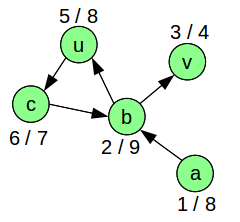
\includegraphics[height=5cm]{aufg7}
\end{figure}
\end{document}